\section{Introduction }
\label{sec:introduction}

\subsection{Background}
\label{subsec:background}

A rumor is defined as a ``proposition for belief of topical reference disseminated without official verification,''~\cite{knapp-1944} a notion that lends itself quite well to the imagination of applied mathematicians.
The mathematics of rumor spread is somewhat explored, beginning with the epidemic model applied to information spread in a population by Daley and Kendall in 1965.
This model's assumptions of homogeneous interactions and its lack of well-defined parameters likely caused ``the superficial similarity between rumors and epidemics to break down on closer scrutiny''~\cite{daley-1965}.
Nonetheless, the similarities of knowing and spreading a rumor, and having and spreading a disease, share parallels that only deviate in some of the intricacies of their mechanism.
In both, an ``infected'' individual in a network desires to (or inadvertently spreads) their ``condition.''
With disease, one of the mechanisms of suppressing spread is vaccination; with rumors it is an individual's eventual boredom and desire for novel information.

More recent models of rumor spread in a population examined the dynamics through randomized networks~\cite{karp-2000}, examining the rumor transmission in exponentially distributed networks~\cite{moreno-2004}, and the time of rumor spread given contacts of the initial spreader in a regular network~\cite{fount-2010}.
There is increasing emphasis on the structure of networks themselves and how this affects model dynamics~\cite{zhang-2013, pellis-2015, pellis-2012, ball-2010, zhou-2007}.
Many of these models derive their structure and dynamics from complex yet internally homogeneous simulations of how individuals interact with rumors.
However, with the advent of massive social media networks that allow sharing of information on a large scale, more analyses are focusing on behaviors (such as rumors) that are frequent in social media networks.
Simulations of rumor spread through social media are becoming increasingly realistic by including ``forgetting'' mechanisms typical of social media~\cite{zhao-2011}, comparing time of rumor spread in random networks as compared to structured networks~\cite{liu-2011}, methods for combatting rumor spread in social networks~\cite{tripathy-2010}, and examining rumor spread on gaming networks~\cite{grab-2008}.

\subsection{The ISTK Model}
\label{subsec:istk}

In this paper we consider a stochastic rumor spread model with four categories of individuals: the ``ignorant'' individuals, those who have never heard the rumor; the ``spreaders,'' those that have heard the rumor and are actively spreading it; the ``stiflers,'' those who have heard the rumor and actively suppress further transmission (either because they now consider the rumor old news, or they never believed the rumor in the first place); and finally the ``knowledgeable'' population, those who have heard, but have subsequently forgotten the rumor.
The rumor initializes in only a small fraction of the population, and spreads as the individuals interact.
The ``ignorant,'' ``spreader,'' and ``stifler'' populations were presented in the Daley-Kendall model~\cite{daley-1965}, but we have added a ``knowledgeable'' population, which has been postulated before as necessarily distinct from the ignorant population~\cite{zhao-2012, zhao-2011}.
Assuming otherwise presumes that the attitude of an individual who has forgotten a rumor is identical to the behavior of an individual who had not yet heard the rumor.
We account for this distinction with the addition of the knowledgeable population to the Daley-Kendall model.
This model is henceforth referred to as the Ignorant, Spreader, Stifler, and Knowledgeable (ISTK) model.
We use three variations of this model: one differential, and two agent-based.
The differential ISTK model simulates a homogenous group of people, and has no awareness of the concept of individuals; it simply ``moves'' proportions of the group of people from one population to another over time.
The first agent-based model, the ``Simple model,'' simulates individuals through several iterations (rounds) over time.
The model incorporates a network that represents the connections between individuals, which in this case is based off of Facebook friends.
The second agent-based model, the ``Feature-vector model,'' incorporates demographic data of these Facebook users.

In the ``Feature vector model,'' we further consider 1.\ how a rumor might be targeted towards a certain demographic, and 2.\ how the ``similarity'' between a rumor and an individual affect a user's behavior.
The original social network dataset included many different types of ``features:'' education level, gender, and language.
Instead of assuming that every individual is equally likely to spread any rumor, we assumed that the rumor's targeted characteristics and the demographic information of each individual affected the likelihood of the rumor to spread.
In this way, we equipped the rumor with a \textit{personality}.
If the individual from whom they heard the rumor was more similar to them, they were more likely to believe the rumor, and if the rumor's characteristics was more similar to theirs they were more likely to spread the rumor.
There is evidence to suggest that people are more likely to believe information that comes from others with similar values~\cite{gillespie-2004}.
The similarity of the rumor's personality to that of the individual's influenced the individual's probability to spread the rumor.
The theory of confirmation bias suggests this behavior, insofar as we are more likely to accept information that confirms our previous beliefs~\cite{wason-1960}.
The characteristics of the rumor itself contribute to how the rumor is spread between individuals in the Feature vector model, Section~\ref{subsec:fvmodelsetup}.

\subsection{ISTK Model Equations}
\label{subsec:istkeqns}

\begin{figure}[H]
\captionsetup{width=0.6\textwidth}
\centering
    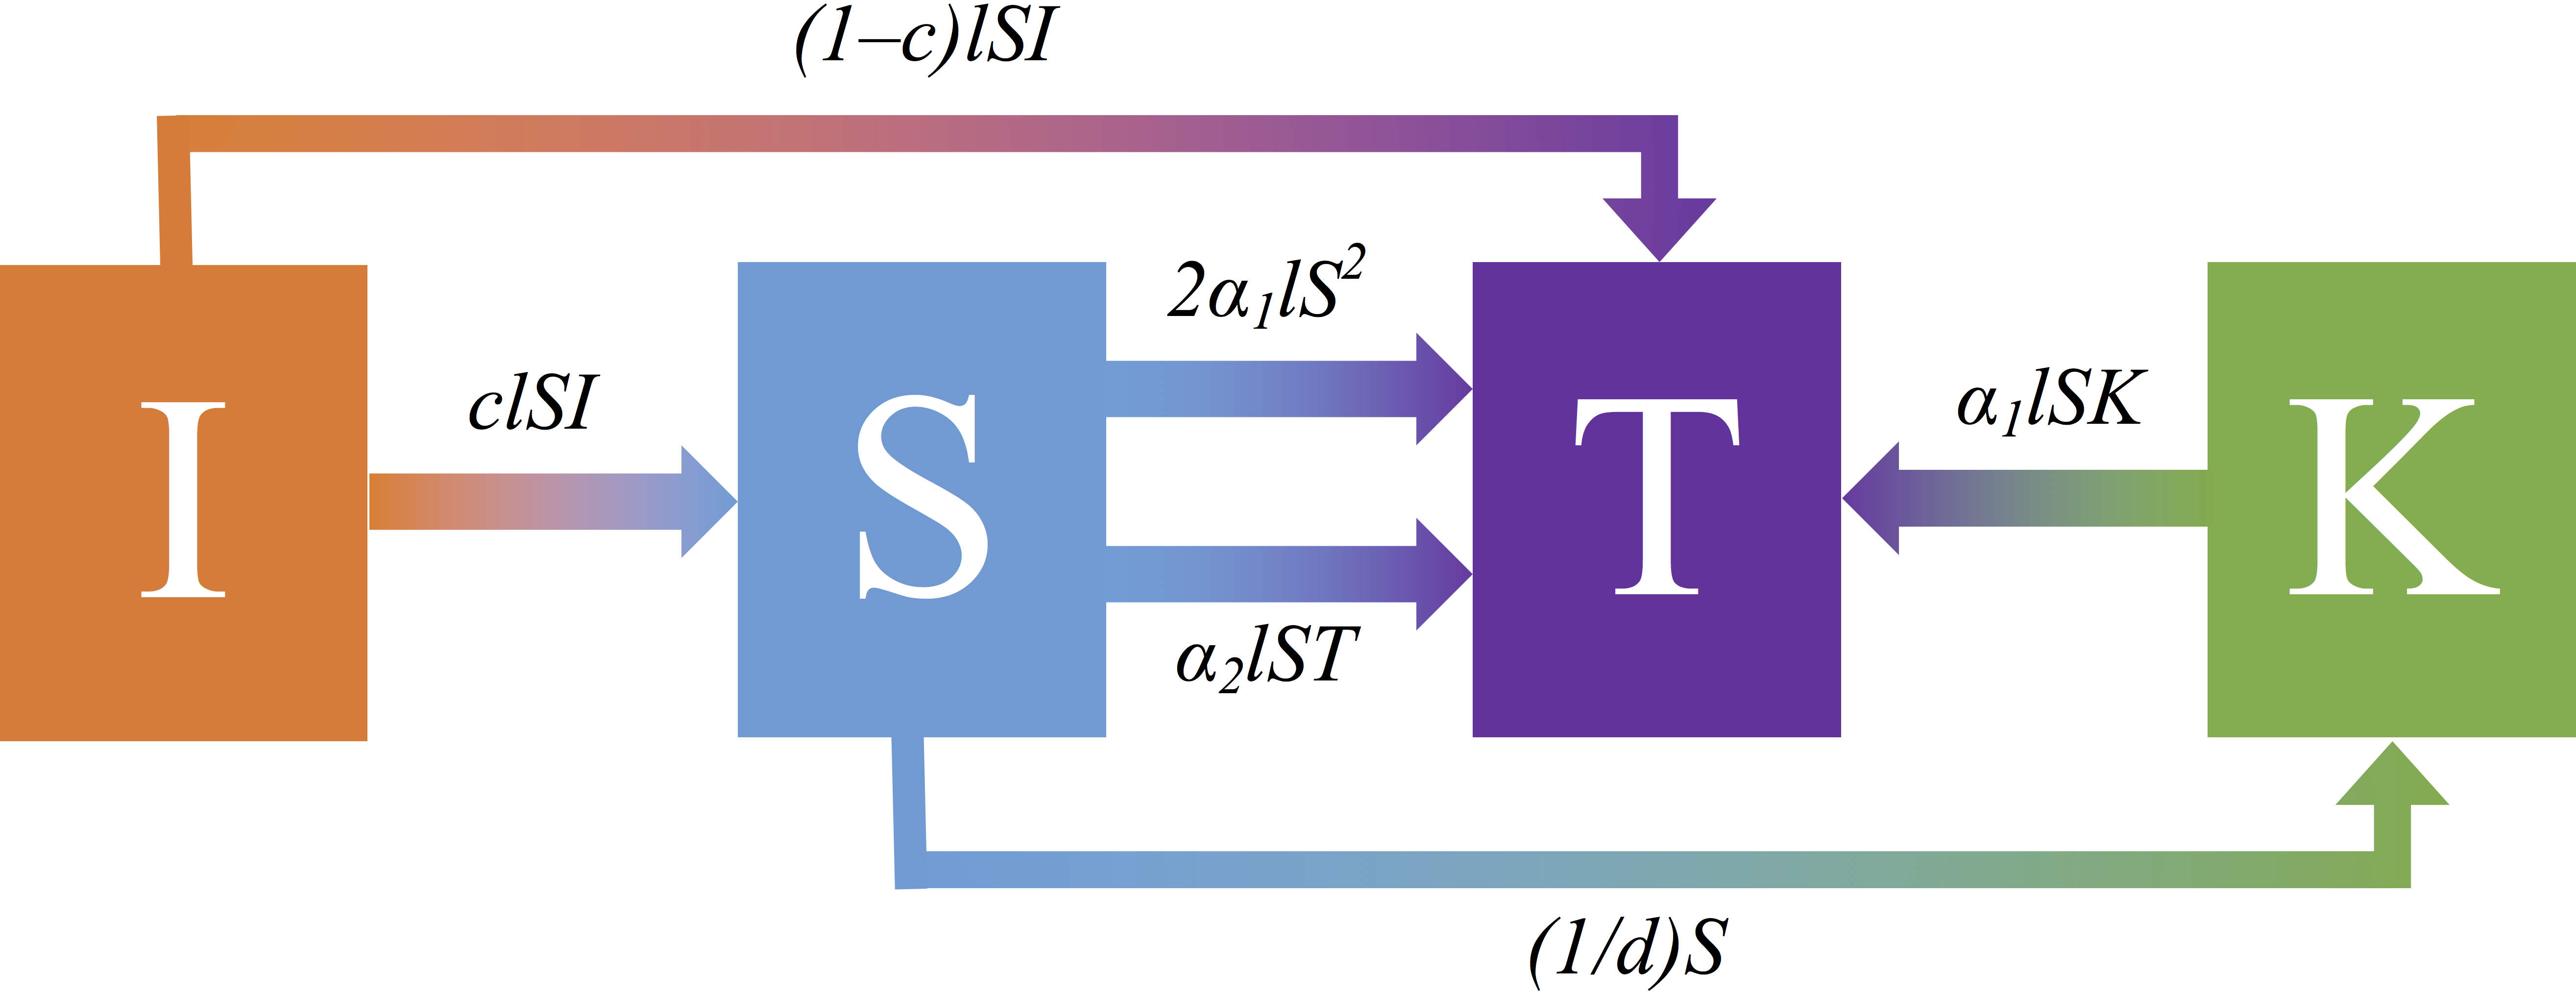
\includegraphics[width=0.85\textwidth]{figures/flow-chart}
  \caption{ ISTK Model}
\label{fig:flow-chart}
\end{figure}

\noindent $ I $, $ S $, $ T $, and $ K $, represent the total Ignorant, Spreader, Stifler, and Knowledgeable populations respectively.
We also designate $ N $ to represent the total size of the population, in that $ N = I + S + T + K $ (n.b.\ we assume no one dies or is born, so N stays constant, i.e. $\frac{dN}{dt} = 0$).

There are several common parameters to all four differential equations, as follows:

We represent the ``credibility'' of the rumor, expressed as a probability that the Ignorant believes the Spreader, as $ c $.
Therefore $ (1 - c) $\, the complement of $ c $ is equivalent to being incredulous of the rumor.

To represent the chance per day of interaction, $ l $, we take the complement of the overall probability that an individual does not talk with a single Spreader.
It is computed by a set of Bernoulli trials with success probability $ \rho $ where $ \rho = 1 - \frac{S}{N} $ and number of trials to be $ \tau $ (i.e.~$ l = 1 - \rho^\tau $).

$ d $ represents the number of days after which a population spontaneously forgets a rumor.
$\alpha_1$ that describes the loss of novelty of the rumor.
$ \alpha_2 $ describes the chance that the Spreader becomes a Stifler upon interacting with a Stifler.

The equations for each population follow:

\begin{equation}
\label{eqn:istk_exp_i}
\frac{dI}{dt} = - clSI - (1-c)lSI \\
\end{equation}

In Equation~\ref{eqn:istk_exp_i}, the first term describes the interaction between an Ignorant and a Spreader.
It is dependent on both the size of the Ignorant and Spreader classes, and is proportional to parameters $ c $ and $ l $.
 The second term of Equation~\ref{eqn:istk_exp_i} accounts for the complement of ``believing the rumor'' (being ``incredulous'' of the rumor) and is proportionate to $ (1 - c) $.
Both terms remove some of the population from the Ignorant class and lead to the Spreader class and Stifler class respectively. Although we can simplify this equation to ($-lSI$), we want to distinguish the credulous ($ c $) and incredulous ($ 1 - c $) group of people.

\begin{equation}
\label{eqn:istk_exp_s} \frac{dS}{dt} = clSI - \frac{1}{d} S - 2 \alpha_1l S^2 - \alpha_2 ST \\
\end{equation}

The first term of Equation~\ref{eqn:istk_exp_s} is the addition of members from the Ignorant class who believed the rumor.
The second term characterizes the population which spontaneously forgets the rumor, and hence is inversely proportionate to the Spreader population and $ d $.
The third term of Equation~\ref{eqn:istk_exp_s} accounts for two Spreaders who interact with each other and foster disinterest in the rumor (since the rumor has lost its novelty).
When these two Spreaders interact ($S^2$), we account for the chance that \textbf{each} Spreader could become a Stifler by multiplying the term by $ 2 $.
The final term represents the disillusionment power of a Stifler when interacting with a Spreader.

\begin{equation}
\label{eqn:istk_exp_t} \frac{dT}{dt} = 2 \alpha_1l S^2 + \alpha_1l SK + \alpha_2 ST + (1-c)lSI \\
\end{equation}

In equation~\ref{eqn:istk_exp_t}, the first of which describes the removal of members from the Spreader class into the Stifler as defined above.
The second term describes the population of Knowledgeable individuals who become a Stifler, as described in Equation~\ref{eqn:istk_exp_s}.
The third and fourth terms of Equation~\ref{eqn:istk_exp_t} describe the addition of members to the Stifler population from the Spreader and Ignorant populations, respectively.

\begin{equation}
\label{eqn:istk_exp_k} \frac{dK}{dt} = \frac{1}{d}S - \alpha_1l SK
\end{equation}

Finally, Equation~\ref{eqn:istk_exp_k} describes the individuals in the Spreader class who forget the rumor and become Knowledgeable; and the population which loses the novelty of the rumor and become Stiflers.

In our model, we do not consider the interaction between a Stifler and an Ignorant because neither one has a reason to broach the subject of a rumor (the Ignorant because they do not know and the Stifler because they no longer care).
Moreover, by a similar logic, when a Knowledgeable and Stifler interact, there is no change in populations.


Our equation differs from the Daley-Kendall model~\cite{daley-1965} primarily through addition of the Knowledgeable class, individuals in this category would have been in the Ignorant of Stifler classes in the original model.
In addition, the Daley-Kendall model assumes all individuals who hear a rumor will believe it.
In our case, this is not so, through addition of the parameter $ c $.
In the Daley-Kendall model it is possible to become ignorant after hearing the rumor, and in this case that is not possible.
